% --------------------------------------------------------------
% This is all preamble stuff that you don't have to worry about.
% Head down to where it says "Start here"
% --------------------------------------------------------------
 

% --------------------------------------------------------------
%                         Start here
% --------------------------------------------------------------
 
%\renewcommand{\qedsymbol}{\filledbox}

\title{TUTORIAL 6}%replace X with the appropriate number
\author{TRISTAN GLATARD\\ %replace with your name
COMP 361 Numerial Methods} %if necessary, replace with your course title
\date{October 26, 2018} 
\maketitle

\begin{exercise}{1} %You can use theorem, proposition, exercise, or reflection here. 
Use the recursive trapezoidal rule to evaluate $ \int_0^{\frac{\pi}{4}} ln(1 + tan x)dx.$ Explain the results.

\textbf{Solution.} 

The recursive trapezoidal formulas for each iteration are:
Iteration 1:
\begin{align}
I_1=[f(a)+f(b)]\frac{H}{2} \notag
\end{align}
where 
\begin{align}
a&=0 \notag \\
b&=\frac{\pi}{4} \notag \\
H&=b-a=\frac{\pi}{4} \notag \\
\end{align}
Thus,
\begin{align}
I_1&=[ln(1+tan(0))+ln(1+tan(\frac{\pi}{4}))]\frac{\pi}{8} \notag \\
&\approx 0.2722 \notag
\end{align}
Iteration 2:
\begin{align}
I_2&=[f(a)+2f(a+\frac{H}{2})+f(b)]\frac{H}{4} \notag \\
&=[ln(1+tan(0))+2ln(1+tan(\frac{\pi}{8}))+ln(1+tan(\frac{\pi}{4}))]\frac{\pi}{16} \notag \\
&\approx 0.2722 \notag
\end{align}
Here we stop the iteration as $\vert I_2 - I_1\vert < \epsilon$.
This result means we only need one iteration for the recursive trapezoidal algorithm to converge. In other words, first approximation is already good enough.
This is intuitive if we look at the plot of f(x) = ln(1+tanx) on the interval \([0,\frac{\pi}{4}]\)

\textit{Hint: type \textbf{ln(1+tan(x))} on google search bar and it draws the plot for you.}

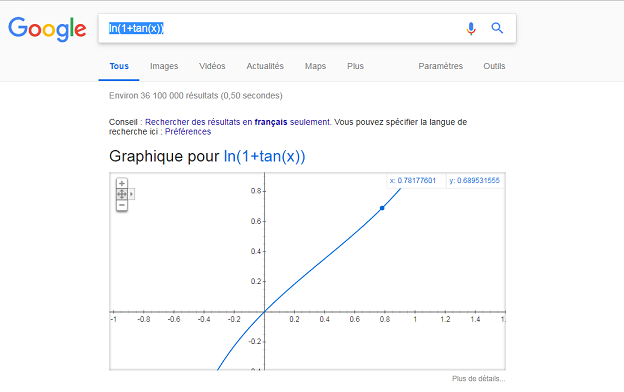
\includegraphics[]{plot_ln(1+tanx).png}

The plot looks very close to a line in that interval. Remember that with \textit{trapezoid} method, we approximate the function to a line so that the integral is approximated to the area of a trapezoid. That's why we have very close approximation right on first iteration.
\end{exercise}

%EXERCISE 2-----------------------------------------------------
\begin{exercise}{2} %You can use theorem, proposition, exercise, or reflection here.  
Evaluate $I=\int_{-1}^1 cos(2cos^{-1}x)dx$ with Simpson’s 1/3 rule using two, four, and six
panels. Explain the results.

\textbf{Solution.}

\textit{Note: just to make the notation clear, $cos^{-1}x$ denotes the arccosine function of \(x\) , not the power function.}

In this problem, \(a=-1, b=1\)

With two panels, let's denote $h= h_2=\frac{b-a}{2}=1$  we have three points at \([-1,0,1]\)

Then, the approximation using Simpson's 1/3 rule is
\begin{align}
I \approx I_2 &= \left[f(a) + 4f(\frac{a+b}{2}) + f(b)\right]\frac{h}{3} \notag \\
&=\left[cos(2*cos^{-1}(-1))+4cos(2*cos^{-1}(0)) + cos(2*cos^{-1}(1))\right]\frac{1}{3} \notag \\
&\approx -0.6666 \notag
\end{align}

With four panels, let's denote \(h= h_4=\frac{b-a}{4}=0.5\) we have two intervals to apply Simpson's 1/3 rule: three points at \([-1,-0.5,0]\) and another three points at \([0,0.5,1]\)
Then, the approximation using Simpson's 1/3 rule is
\begin{align}
I \approx I_4 &= \left[cos(2*cos^{-1}(-1))+4cos(2*cos^{-1}(-0.5)) + cos(2*cos^{-1}(0))\right]\frac{0.5}{3} \notag \\
&+ \left[cos(2*cos^{-1}(0))+4cos(2*cos^{-1}(0.5)) + cos(2*cos^{-1}(1))\right]\frac{0.5}{3} \notag \\
&\approx -0.6666 \notag
\end{align}

With six panels, let's denote \(h= h_6=\frac{b-a}{6}=0.3333\) we have three intervals to apply Simpson's 1/3 rule: three points at \([-1,-0.6666,-0.3333]\), \([-0.3333,0,0.3333]\) and another three points at \([0.3333,0.6666,1]\)
Then, the approximation using Simpson's 1/3 rule is
\begin{align}
I \approx I_6 &= \left[cos(2*cos^{-1}(-1))+4cos(2*cos^{-1}(-0.6666)) + cos(2*cos^{-1}(-0.3333))\right]\frac{0.3333}{3} \notag \\
&+ \left[cos(2*cos^{-1}(-0.3333))+4cos(2*cos^{-1}(0)) + cos(2*cos^{-1}(0.3333))\right]\frac{0.3333}{3} \notag \\
&+ \left[cos(2*cos^{-1}(0.3333))+4cos(2*cos^{-1}(0.6666)) + cos(2*cos^{-1}(1))\right]\frac{0.3333}{3} \notag \\
&\approx -0.6666 \notag
\end{align}
We can see that Simpson's rule seems to give the same approximation for two, four and six panels. 
Let's see how by looking at the plot of the function.

\textit{Hint: mathisfun.com has a cool widget that lets you approximate (and see plots) integrals of any functions of your choice.}

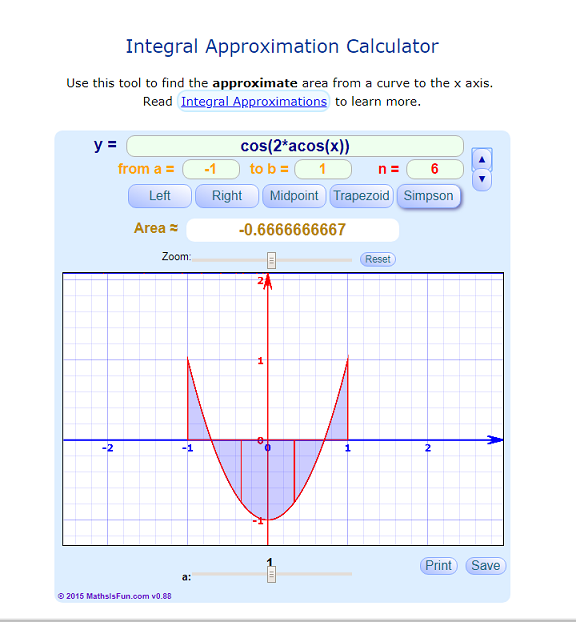
\includegraphics[]{cos(2acos(x)).png}


In the plot, we can the that the function \(cos(2*cos^{-1}(x))\) is a parabola. Remember that Simpson's 1/3 rule is derived from Newton-Cotes formulas with n = 2; that is, by passing a parabolic interpolant through three adjacent nodes. Because parabolic interpolation is unique with three points, we get exact results regardless of number of panels.
\end{exercise}


%EXERCISE 3-----------------------------------------------------
\begin{exercise}{3} %You can use theorem, proposition, exercise, or reflection here.  
The following table gives the pull F of the bow as a function of the draw x. If the bow is drawn 0.5m, determine the speed of the 0.075-kg arrow when it leaves the bow. Hint: The kinetic energy of the arrow equals the work done in drawing the bow; that is, $mv^2/2 = \int_0^{0.5m} Fdx$
\begin{table}[h]
\centering
\begin{tabular}{|c|c|c|c|c|c|c|c|c|c|c|c|}
\hline
x(m) &0.00& 0.05& 0.1& 0.15& 0.20 & 0.25&0.30&0.35&0.40&0.45&0.50\\ \hline
F(N)& 0& 37& 71 &104 &134 &161 &185& 207& 225& 239& 250 \\ \hline
\end{tabular}
\end{table}

\textbf{Solution.} 

In this problem, we have 11 evenly-spaced data points (or, 10 panels) with \(h=0.05\).
So we can approximate the integral  $\int_0^{0.5m} Fdx$ by applying Simpson's 1/3 rule on five pairs of panels:
On \([0,0.05,0.1]\)
 \begin{align}
 I_{0,0.1} &\approx \left[F(0) + 4F(0.05) + F(0.1)\right]\frac{0.05}{3} \notag \\
 &=(0+4*37+71)\frac{0.05}{3} = 3.65 \notag
 \end{align}
On \([0.1,0.15,0.2]\)
 \begin{align}
 I_{0.1,0.2} &\approx \left[F(0.1) + 4F(0.15) + F(0.2)\right]\frac{0.05}{3} \notag \\
 &=(71+4*104+134)\frac{0.05}{3} = 10.35 \notag
 \end{align}
On \([0.2,0.25,0.3]\)
 \begin{align}
 I_{0.2,0.3} &\approx \left[F(0.2) + 4F(0.25) + F(0.3)\right]\frac{0.05}{3} \notag \\
 &=(134+4*161+185)\frac{0.05}{3} = 16.05 \notag
 \end{align}
On \([0.3,0.35,0.4]\)
 \begin{align}
 I_{0.3,0.4} &\approx \left[F(0.3) + 4F(0.35) + F(0.4)\right]\frac{0.05}{3} \notag \\
 &=(185+4*207+225)\frac{0.05}{3} = 20.63 \notag
 \end{align}
On \([0.4,0.45,0.5]\)
 \begin{align}
 I_{0.4,0.5} &\approx \left[F(0.4) + 4F(0.45) + F(0.5)\right]\frac{0.05}{3} \notag \\
 &=(225+4*239+250)\frac{0.05}{3} = 23.85 \notag
 \end{align}
 Then,
 \begin{align}
 I=\sum I_{i,i+2}&= I_{0,0.1}+I_{0.1,0.2}+I_{0.2,0.3}+I_{0.3,0.4}+I_{0.4,0.5}\notag \\
 &\approx 3.65 + 10.65 + 16.05+20.63 + 23.85 \notag \\
 &=74.83 \notag
 \end{align}
 Now the speed of the arrow would be
 
 \begin{align}
 v&=\sqrt{\frac{2I}{m}} \notag \\
 &=\sqrt{\frac{2*74.83}{0.075}} \notag \\
 &\approx 44.67 \notag
 \end{align}
 \end{exercise}

\begin{exercise}{4} Evaluate $\int_1^\pi \frac{ln(x)}{x^2-2x+2}dx$
with Gauss-Legendre quadrature. Use (a) two nodes; and (b) four nodes.

\textbf{Solution}
First we need to "transform" the integration range \([1,\pi]\) to the one required by Gauss-Legendre quadrature \([-1,1]\).
\begin{align}
x&=\frac{b+a}{2} + \frac{b-a}{2}\xi \notag \\
&=\frac{\pi+1}{2} + \frac{\pi-1}{2}\xi \notag
\end{align}
\end{exercise}
Now \(dx = d\xi \frac{b-a}{2}\), and the quadrature becomes
\begin{align}
\int_1^\pi \frac{ln(x)}{x^2-2x+2}dx = \frac{\pi-1}{2} \sum_0^n A_if(x_i)
\end{align}
a) With two nodes, we have the following table of calculation (see Table 6.3 on Kiusalaas 2011)

\begin{table}[h]
\centering
\begin{tabular}{|r|r|r|r|r|}
\hline
\multicolumn{1}{|c|}{\textit{\textbf{\(\xi_i\)}}} & \multicolumn{1}{c|}{\textit{\textbf{\(x_i\)}}} & \multicolumn{1}{l|}{\textit{\(f(x_i\))}} & \multicolumn{1}{l|}{\textit{\(A_i\)}} & \multicolumn{1}{l|}{\textit{\(A_i*f(x_i)\)}} \\ \hline
-0.577350 & 1.452572 & 0.309868 & 1.000000 & 0.309868 \\ \hline
0.577350 & 2.689021 & 0.256743 & 1.000000 & 0.256743 \\ \hline
\end{tabular}
\caption{Abscissas and weights for Gauss-Legendre, n=1}
\label{tab-gauss-legendre-2-nodes}
\end{table}

Then we have approximation
\begin{align}
I&\approx\frac{\pi-1}{2} \sum_0^1 A_if(x_i) \notag \\
&=\frac{3.141593-1}{2} (0.309868+0.256743) \notag \\
&=0.606725 \notag
\end{align}
b) Now with four nodes, we have the following table of calculation

\begin{table}[h]
\centering
\begin{tabular}{|r|r|r|r|r|}
\hline
\multicolumn{1}{|c|}{\textit{\textbf{\(\xi_i\)}}} & \multicolumn{1}{c|}{\textit{\textbf{\(x_i\)}}} & \multicolumn{1}{l|}{\textit{\(f(x_i\))}} & \multicolumn{1}{l|}{\textit{\(A_i\)}} & \multicolumn{1}{l|}{\textit{\(A_i*f(x_i)\)}} \\ \hline
-0.339981 & 1.706746 & 0.356514 & 0.652145 & 0.232499 \\ \hline
-0.861136 & 1.148695 & 0.135628 & 0.347855 & 0.047179 \\ \hline
0.339981 & 2.434847 & 0.290927 & 0.652145 & 0.189727 \\ \hline
0.861136 & 2.992898 & 0.220499 & 0.347855 & 0.076702 \\ \hline\end{tabular}
\caption{Abscissas and weights for Gauss-Legendre, n=3}
\label{tab-gauss-legendre-4-nodes}
\end{table}
Then we have approximation
\begin{align}
I&\approx\frac{\pi-1}{2} \sum_0^3 A_if(x_i) \notag \\
&=\frac{3.141593-1}{2} (0.232499+0.047179+0.189727+0.076702) \notag \\
&=0.584768 \notag
\end{align}



% --------------------------------------------------------------
%     You don't have to mess with anything below this line.
% --------------------------------------------------------------
 